\chapter{Estado del Arte}

En este capítulo hablaremos sobre la situación de la industria del entretenimiento digital hoy en día, qué es un \textit{roguelike}, los elementos que dificultan y facilitan el uso de diferentes programas y \textit{software} a ciertos sectores de la sociedad como invidentes o daltónicos, qué opciones de accesibilidad existen en diferentes sistemas operativos y las razones por las que hemos elegido ciertas de las características de las que queremos dotar a nuestro proyecto.

\section{La industria del entretenimiento digital en la actualidad}

Desde sus primeros pasos hasta hoy en día, tal y como sucede con muchas de las novedades en el mundo del entretenimiento y la cultura, el sector del ocio digital ha sufrido cierto estigma por una gran parte de la población, siendo censurado y degragado en mayor o menor medida, no tan solo por cierta parte de la sociedad, pero también por muchos medios de comunicación y gobiernos. A pesar de que hoy en día este problema todavía está activo\footnote{Es común que cada año en Australia se censuren algunos juegos como \href{http://goo.gl/hFrQah}{Paranautical Activity} por razones que otras formas de entretenimiento y cultura como películas o libros no se ven tan afectados.}, la industria se ha expandido tanto (consolas, ordenadores, navegadores, Facebook, móvil...), que cada vez es más complicado encontrar a alguien que no haya jugado a algún videojuego en las últimas semanas y ya es algo que forma parte del día a día de mucha parte de la población.

\subsection{La industria, en números}
En todo el mundo, pero especialmente en EEUU, la industria de los videojuegos es uno de los sectores con más crecimiento\footnote{\url{http://www.theesa.com/wp-content/uploads/2014/11/Games_Economy-11-4-14.pdf}} llegando a generar, solamente en ventas digitales, alrededor de 61 billones de dólares en el año 2015\footnote{http://goo.gl/BgGhXy}.

Este gran éxito se debe, en gran parte, a la irrupción de los juegos desarrollados para móviles, cuyo beneficio ha ido aumentando enormemente durante los últimos años. \footnote{\href{http://goo.gl/Lz9UAa}{La venta de videojuegos en Alemania crece año tras año, pero el mayor aumento de beneficio se está centrando en el mercado de los juegos para móvil}}. Sin embargo, esto no significa que el resto de plataformas no estén triunfando. Solamente Steam, la plataforma de distribución digital para PC por excelencia desarrollada por Valve, ha generado alrededor de 3 billones y medio de dólares en el año 2015\footnote{\url{http://goo.gl/Mbjgol}}.

Con el mercado del PC resurgiendo, las consolas de sobremesa obteniendo grandes números de ventas, las portátiles resistiendo, el mercado de los videojuegos para móvil en esplendor y los cascos de realidad virtual llegando al mercado este año 2016; todo parece indicar que estos números no harán más que crecer en los próximos años.

\subsection{Conclusión}

Lo que comenzó hace varias décadas como un modo de entretenimiento sin ninguna pretensión, generalmente enfocado a adolescentes y que miraba a otras industrias como la cinematográfica con recelo, se ha convertido en todo lo que había deseado y más. Gracias a grandes títulos y a su expansión a toda clase de dispositivos, no se puede hablar de la industria del entretenimiento sin hablar de videojuegos y en muchos casos algunos de esos títulos han logrado ser nombrados como obras de arte en su género, pasando a la historia y siendo recordados a lo largo de los años.

Sin embargo, es bastante probable que lo mejor esté todavía por llegar.

\section{\textit{Roguelikes.}}

\subsection{Qué es y orígenes}

En 1983, Michael Toy y Glenn Wichman crearon un videojuego llamado Rogue\footnote{Desde 2014 este juego se encuentra disponible en \href{https://archive.org/details/msdos_Rogue_1983}{archive.org}} que acabó defiendo un género.

Las características principales que definieron a Rogue y que, por extensión, definieron al género de los \textit{roguelikes} inicialmente, son:

\paragraph{Dificultad}: Rogue es un videojuego difícil que obligará al jugador a rejugarlo una y otra vez, intentando llegar más lejos que la anterior vez gracias a ir aprendiendo los funcionamientos del mismo.

\paragraph{Aleatoriedad}: Cada vez que el jugador comienza una partida nueva se encontrará con ciertos elementos que han cambiado con respecto a la anterior: el mapa es diferente, los elementos y enemigos se encuentran en sitios distintios, los propios objetos han cambiado... causando que cada partida tenga un grado de dificultad pseudo-aleatorio dependiendo de la semilla con la que estos elementos han sido generados.

\paragraph{Progresión}: Una de las frases más escuchadas en las críticas que Rogue recibió tras su lanzamiento es que el jugador sentía la necesidad de intentar llegar más lejos en cada ocasión\footnote{Jerry Pournelle habló de ello en \href{http://goo.gl/Iz2qg6}{este artículo}}. Esto viene dado, sobre todo, por la sensación de progresión y de que en cada \textit{run}\footnote{Palabra comúnmente usada en estos géneros y que se refiere a una partida desde su inicio hasta que el jugador pierde} el jugador va mejorando.  

\begin{figure}[h!]
		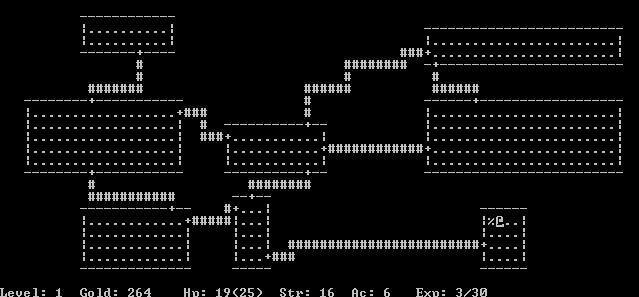
\includegraphics[width=\textwidth,height=\textheight,keepaspectratio]{C:/Users/Dario/Documents/GitHub/roomsgamedoc/img/roguegame.PNG}
	\caption{Screenshot de \href{https://en.wikipedia.org/wiki/File:Rogue_Unix_Screenshot_CAR.PNG}{dominio público} del videojuego Rogue}
	\label{fig:roguegame}
\end{figure}

\subsection{En la actualidad}

\subsection{Elementos \textit{roguelike} en nuestro proyecto}